\documentclass{ximera}

%\usepackage{todonotes}

\newcommand{\todo}{}


\graphicspath{
{./}
{../functionsOfSeveralVariables/}
{../normalVectors/}
{../lagrangeMultipliers/}
}


\usepackage{tkz-euclide}
\tikzset{>=stealth} %% cool arrow head
\tikzset{shorten <>/.style={ shorten >=#1, shorten <=#1 } } %% allows shorter vectors

\usetikzlibrary{backgrounds} %% for boxes around graphs
\usetikzlibrary{shapes,positioning}  %% Clouds and stars
\usetikzlibrary{matrix} %% for matrix
\usepgfplotslibrary{polar} %% for polar plots
\usetkzobj{all}
\usepackage[makeroom]{cancel} %% for strike outs
%\usepackage{mathtools} %% for pretty underbrace % Breaks Ximera
\usepackage{multicol}





\usepackage{array}
\setlength{\extrarowheight}{+.1cm}   
\newdimen\digitwidth
\settowidth\digitwidth{9}
\def\divrule#1#2{
\noalign{\moveright#1\digitwidth
\vbox{\hrule width#2\digitwidth}}}





\newcommand{\RR}{\mathbb R}
\newcommand{\R}{\mathbb R}
\newcommand{\N}{\mathbb N}
\newcommand{\Z}{\mathbb Z}

\newcommand{\sage}{\textsf{SageMath}}


%\renewcommand{\d}{\,d\!}
\renewcommand{\d}{\mathop{}\!d}
\newcommand{\dd}[2][]{\frac{\d #1}{\d #2}}
\newcommand{\pp}[2][]{\frac{\partial #1}{\partial #2}}
\renewcommand{\l}{\ell}
\newcommand{\ddx}{\frac{d}{\d x}}

\newcommand{\zeroOverZero}{\ensuremath{\boldsymbol{\tfrac{0}{0}}}}
\newcommand{\inftyOverInfty}{\ensuremath{\boldsymbol{\tfrac{\infty}{\infty}}}}
\newcommand{\zeroOverInfty}{\ensuremath{\boldsymbol{\tfrac{0}{\infty}}}}
\newcommand{\zeroTimesInfty}{\ensuremath{\small\boldsymbol{0\cdot \infty}}}
\newcommand{\inftyMinusInfty}{\ensuremath{\small\boldsymbol{\infty - \infty}}}
\newcommand{\oneToInfty}{\ensuremath{\boldsymbol{1^\infty}}}
\newcommand{\zeroToZero}{\ensuremath{\boldsymbol{0^0}}}
\newcommand{\inftyToZero}{\ensuremath{\boldsymbol{\infty^0}}}



\newcommand{\numOverZero}{\ensuremath{\boldsymbol{\tfrac{\#}{0}}}}
\newcommand{\dfn}{\textbf}
%\newcommand{\unit}{\,\mathrm}
\newcommand{\unit}{\mathop{}\!\mathrm}
\newcommand{\eval}[1]{\bigg[ #1 \bigg]}
\newcommand{\seq}[1]{\left( #1 \right)}
\renewcommand{\epsilon}{\varepsilon}
\renewcommand{\iff}{\Leftrightarrow}

\DeclareMathOperator{\arccot}{arccot}
\DeclareMathOperator{\arcsec}{arcsec}
\DeclareMathOperator{\arccsc}{arccsc}
\DeclareMathOperator{\si}{Si}
\DeclareMathOperator{\proj}{\vec{proj}}
\DeclareMathOperator{\scal}{scal}
\DeclareMathOperator{\sign}{sign}


%% \newcommand{\tightoverset}[2]{% for arrow vec
%%   \mathop{#2}\limits^{\vbox to -.5ex{\kern-0.75ex\hbox{$#1$}\vss}}}
\newcommand{\arrowvec}{\overrightarrow}
%\renewcommand{\vec}[1]{\arrowvec{\mathbf{#1}}}
\renewcommand{\vec}{\mathbf}
\newcommand{\veci}{{\boldsymbol{\hat{\imath}}}}
\newcommand{\vecj}{{\boldsymbol{\hat{\jmath}}}}
\newcommand{\veck}{{\boldsymbol{\hat{k}}}}
\newcommand{\vecl}{\boldsymbol{\l}}
\newcommand{\utan}{\mathbf{\hat{t}}}
\newcommand{\unormal}{\mathbf{\hat{n}}}
\newcommand{\ubinormal}{\mathbf{\hat{b}}}

\newcommand{\dotp}{\bullet}
\newcommand{\cross}{\boldsymbol\times}
\newcommand{\grad}{\boldsymbol\nabla}
\newcommand{\divergence}{\grad\dotp}
\newcommand{\curl}{\grad\cross}
%\DeclareMathOperator{\divergence}{divergence}
%\DeclareMathOperator{\curl}[1]{\grad\cross #1}
\newcommand{\lto}{\mathop{\longrightarrow\,}\limits}


\colorlet{textColor}{black} 
\colorlet{background}{white}
\colorlet{penColor}{blue!50!black} % Color of a curve in a plot
\colorlet{penColor2}{red!50!black}% Color of a curve in a plot
\colorlet{penColor3}{red!50!blue} % Color of a curve in a plot
\colorlet{penColor4}{green!50!black} % Color of a curve in a plot
\colorlet{penColor5}{orange!80!black} % Color of a curve in a plot
\colorlet{fill1}{penColor!20} % Color of fill in a plot
\colorlet{fill2}{penColor2!20} % Color of fill in a plot
\colorlet{fillp}{fill1} % Color of positive area
\colorlet{filln}{penColor2!20} % Color of negative area
\colorlet{fill3}{penColor3!20} % Fill
\colorlet{fill4}{penColor4!20} % Fill
\colorlet{fill5}{penColor5!20} % Fill
\colorlet{gridColor}{gray!50} % Color of grid in a plot

\newcommand{\surfaceColor}{violet}
\newcommand{\surfaceColorTwo}{redyellow}
\newcommand{\sliceColor}{greenyellow}




\pgfmathdeclarefunction{gauss}{2}{% gives gaussian
  \pgfmathparse{1/(#2*sqrt(2*pi))*exp(-((x-#1)^2)/(2*#2^2))}%
}


%%%%%%%%%%%%%
%% Vectors
%%%%%%%%%%%%%

%% Simple horiz vectors
\renewcommand{\vector}[1]{\left\langle #1\right\rangle}


%% %% Complex Horiz Vectors with angle brackets
%% \makeatletter
%% \renewcommand{\vector}[2][ , ]{\left\langle%
%%   \def\nextitem{\def\nextitem{#1}}%
%%   \@for \el:=#2\do{\nextitem\el}\right\rangle%
%% }
%% \makeatother

%% %% Vertical Vectors
%% \def\vector#1{\begin{bmatrix}\vecListA#1,,\end{bmatrix}}
%% \def\vecListA#1,{\if,#1,\else #1\cr \expandafter \vecListA \fi}

%%%%%%%%%%%%%
%% End of vectors
%%%%%%%%%%%%%

%\newcommand{\fullwidth}{}
%\newcommand{\normalwidth}{}



%% makes a snazzy t-chart for evaluating functions
%\newenvironment{tchart}{\rowcolors{2}{}{background!90!textColor}\array}{\endarray}

%%This is to help with formatting on future title pages.
\newenvironment{sectionOutcomes}{}{} 



%% Flowchart stuff
%\tikzstyle{startstop} = [rectangle, rounded corners, minimum width=3cm, minimum height=1cm,text centered, draw=black]
%\tikzstyle{question} = [rectangle, minimum width=3cm, minimum height=1cm, text centered, draw=black]
%\tikzstyle{decision} = [trapezium, trapezium left angle=70, trapezium right angle=110, minimum width=3cm, minimum height=1cm, text centered, draw=black]
%\tikzstyle{question} = [rectangle, rounded corners, minimum width=3cm, minimum height=1cm,text centered, draw=black]
%\tikzstyle{process} = [rectangle, minimum width=3cm, minimum height=1cm, text centered, draw=black]
%\tikzstyle{decision} = [trapezium, trapezium left angle=70, trapezium right angle=110, minimum width=3cm, minimum height=1cm, text centered, draw=black]



\outcome{Understand the geometric basis of the method of Lagrange
  multipliers.}

\outcome{Use Lagrange multipliers to solve constrained optimization
  problems.}

\outcome{Define the Lagrangian.}


\title[Dig-In:]{Lagrange multipliers}

\begin{document}
\begin{abstract}
  We give a new method of finding extrema. 
\end{abstract}
\maketitle

Through out this course, we hope it has become apparent that when
given a problem:
\begin{quote}
  \textbf{There is more than one way to solve it.}
\end{quote}
Previously, we were finding extrema of functions $F:\R^n\to\R$ when
constrained to some set $S$.

\begin{example}
  Let $F(x,y) = x^2+3y^2-4x-6y+7$ and let $S$ the set
  \[
  S = \{(x,y):x^2 + y^2 \le 1\}
  \]
  Discuss how to find the maximum and minimum values of $F$ on $S$.
  \begin{explanation}
    To do this we first find the critical points of $F$, that is where
    the components of $\grad F(x,y)$ are zero or do not exist. If
    these points are in $S$, they become candidates for the maxima and
    minima.

    Next we investigate the boundary of $S$. To do this we must
    parameterize the boundary of $S$, or express the boundary either in
    terms of $x$ or $y$. In this case, we can express the boundary
    parametrically as
    \[
    \vec{p}(t) = \vector{\cos(t),\sin(t)},
    \]
    or we could set
    \[
    y = \pm \answer[given]{\sqrt{1-x^2}},
    \]
    or even
    \[
    x = \pm \answer[given]{\sqrt{1-y^2}}.
    \]
  \end{explanation}
\end{example}

Above we see that a crucial step in computing extrema when constrained
to a set is finding an \textbf{explicit formula} for the boundary. This
could be very difficult or even impossible! If our constraining set had been
\[
S = \{(x,y): x+y+\sin(xy) =0\}
\]
our previous method will not work, as we (at least this author!)
cannot find an explicit formula describing the boundary (which in this
case is the set) of the set above. Nevertheless, there is another
way. It is called the method of \textit{Lagrange multipliers}. This
method is named after the mathematician \link[Joesph-Louis
  Lagrange]{http://en.wikipedia.org/wiki/Joseph-Louis_Lagrange}, which
he first employed. This method relies on the \textit{gradient
  vector}. Recall facts about the gradient vector:
\begin{itemize}
\item $\grad F = \vector{\pp[F]{x_1},\pp[F]{x_2},\dots,\pp[F]{x_n}}$.
\item $\grad F(\vec{x})$ points in the direction that one must leave
  $\vec{x}$ in order to see the initial greatest increase in $F$.
\item $\grad F(\vec{x})$ points in the direction that is perpendicular
  to any level surface of $F$.
\end{itemize}

It is this last fact that we will look at now.  Below we see level
curves for some function $F:\R^2\to\R$ along with a constraining curve
that we will call $S$:
\begin{image}
  \begin{tikzpicture}
    \begin{axis}%
      [
        unit vector ratio*=1 1 1,
	ymin=-.2,ymax=4.5,
        width=5in,
	xmin=-4.5,xmax=4.5,
        axis lines=none,
      ]
      \addplot[ultra thick, penColor,smooth,domain=0:180] ({cos(x)},{sin(x)});
      \addplot[ultra thick, penColor,smooth,domain=0:180] ({2*cos(x)},{2*sin(x)});
      \addplot[ultra thick, penColor,smooth,domain=0:180] ({3*cos(x)},{3*sin(x)});
      \addplot[ultra thick, penColor,smooth,domain=0:180] ({4*cos(x)},{4*sin(x)});
      
      \addplot[ultra thick, penColor4,smooth] {x^2+1};      
      
      \node[penColor,fill=white] at (axis cs:-.7,.7) {$7$};
      \node[penColor,fill=white] at (axis cs:-1.4,1.4) {$6$};
      \node[penColor,fill=white] at (axis cs:-2.1,2.1) {$5$};
      \node[penColor,fill=white] at (axis cs:-2.8,2.8) {$4$};

      \node[penColor4] at (axis cs:2,4) {$S$};
      \node[penColor] at (axis cs:-3.8,2) {$F$};
    \end{axis}
  \end{tikzpicture}
\end{image}

Let's add vectors to our graph that point in the direction of $\grad
F(x,y)$. We can do this \textit{without} computation, since we
understand the geometry of the gradient vector, the gradient vector is
perpendicular to level curves:
\begin{image}
  \begin{tikzpicture}
    \begin{axis}%
      [
        unit vector ratio*=1 1 1,
	ymin=-.2,ymax=4.5,
        width=5in,
	xmin=-4.5,xmax=4.5,
        axis lines=none,
      ]
      \addplot[ultra thick, penColor,smooth,domain=0:180] ({cos(x)},{sin(x)});
      \addplot[ultra thick, penColor,smooth,domain=0:180] ({2*cos(x)},{2*sin(x)});
      \addplot[ultra thick, penColor,smooth,domain=0:180] ({3*cos(x)},{3*sin(x)});
      \addplot[ultra thick, penColor,smooth,domain=0:180] ({4*cos(x)},{4*sin(x)});
      
      \addplot[ultra thick, penColor4,smooth] {x^2+1};      
      
      \node[penColor,fill=white] at (axis cs:-.7,.7) {$7$};
      \node[penColor,fill=white] at (axis cs:-1.4,1.4) {$6$};
      \node[penColor,fill=white] at (axis cs:-2.1,2.1) {$5$};
      \node[penColor,fill=white] at (axis cs:-2.8,2.8) {$4$};

      \node[penColor4] at (axis cs:2,4) {$S$};
      \node[penColor] at (axis cs:-3.8,2) {$F$};

      \addplot[penColor2,ultra thick, ->] coordinates{(-1.63,3.65) (-1.22,2.74)};
      \addplot[penColor2,ultra thick, ->] coordinates{(1.63,3.65) (2.04,4.56)};

      \addplot[penColor2,ultra thick, ->] coordinates{(-1.3,2.7) (-.87,1.8)};
      \addplot[penColor2,ultra thick, ->] coordinates{(1.3,2.7) (1.7,3.6)};
      \addplot[penColor2,ultra thick, ->] coordinates{(-.9,1.8) (-.45,.91)};
      \addplot[penColor2,ultra thick, ->] coordinates{(.9,1.8) (1.35,2.7)};
      \addplot[penColor2,ultra thick, ->] coordinates{(0,1) (0,0)};
    \end{axis}
  \end{tikzpicture}
\end{image}

Now we can observe something interesting: If for some point $(x,y)$
the gradient $\grad F(x,y)$ points in the ``general'' direction of the
tangent vectors of $S$, then $(x,y)$ \textbf{cannot} give an extremal
value of $F$, as moving along $S$ will either increase or decrease the
value of $F$. Here's the upshot:
\begin{quote}
  \textbf{The only candidates for local extrema occur when the
    gradient of $F$ is perpendicular to $S$.}
\end{quote}
How do we find these points? To do this, we will imagine that $S$ is a
level curve for some other function $G:\R^2\to\R$, and define $S$ as:
\[
S = \{(x,y):G(x,y)= c\}
\]
now, the candidates for extrema of $F$ when constrained to a curve $S$
are found by finding $(x,y)$ such that
\[
\grad F(x,y) =  \lambda \cdot \grad G(x,y)
\]
since $(x,y)$ that satisfy this equation are those where the gradient
vectors of $F$ are perpendicular to the level curve $G(x,y)= c$. This
is the essence of the method of Lagrange multipliers.

\begin{theorem}[Lagrange Multipliers]
  Let $F:\R^n\to\R$, $G:\R^n\to\R$, $\grad G(\vec{x}) \ne \vec{0}$,
  and let $S$ be the level set
  \[
  S = \{\vec{x}: G(\vec{x}) = c\}
  \]
  If $F$ has extrema when constrained to $S$ at $\vec{x}$, then
  \[
  \grad F(\vec{x}) = \lambda \cdot \grad G(\vec{x})
  \]
  for some number $\lambda$.
\end{theorem}


  


\section{Working with geometry}

Lagrange multipliers tell us that to maximize a function $F:\R^2\to\R$
along a curve defined by $G(x,y) = c$, we need to find where $\grad F$
is perpendicular to $G$. In essence we are detecting geometric
behavior using the tools of calculus.

\begin{example}
  Below we have plotted a curve $G(x,y) = c$ along with $\grad F$.
  \begin{image}
    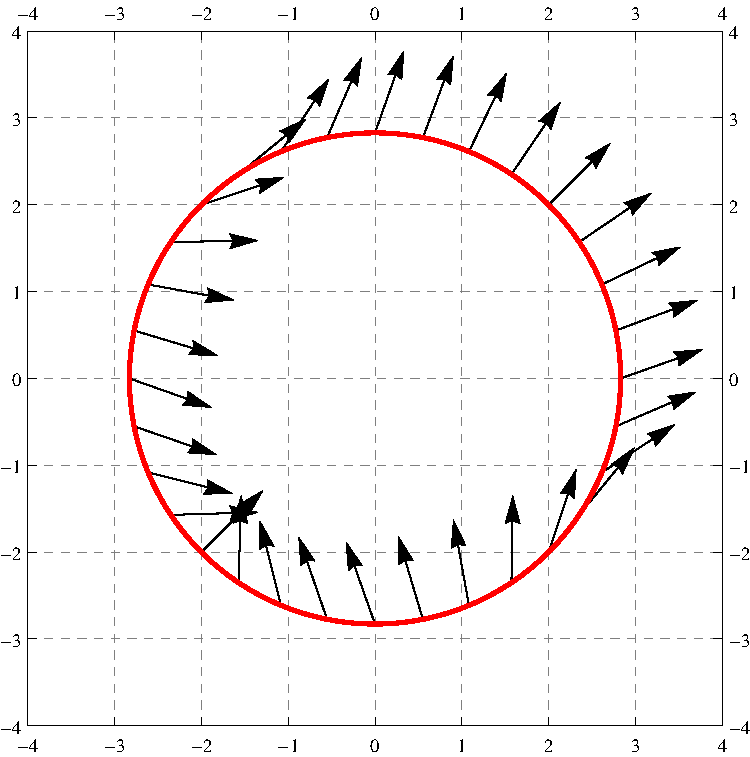
\includegraphics{curveVectors1.pdf}
  \end{image}
  Find the candidates for the maximum and minimum values for $F$ when
  restricted to $G(x,y) = c$.
  \begin{explanation}
    At the candidates for the extrema, we know that the gradient
    vector of $F$ must be
    \wordChoice{\choice{parallel}\choice[correct]{perpendicular}} to
    the curve $G(x,y) = c$. Hence we
    see that the points
    \[
    (x,y) = (\answer[given]{2},2)
    \]
    and
    \[
    (x,y) = (-2,\answer[given]{-2})
    \]
    are our candidates for extrema.
  \end{explanation}
\end{example}

\begin{example}
  Below we have plotted a curve $G(x,y) = c$ along with $\grad F$.
  \begin{image}
    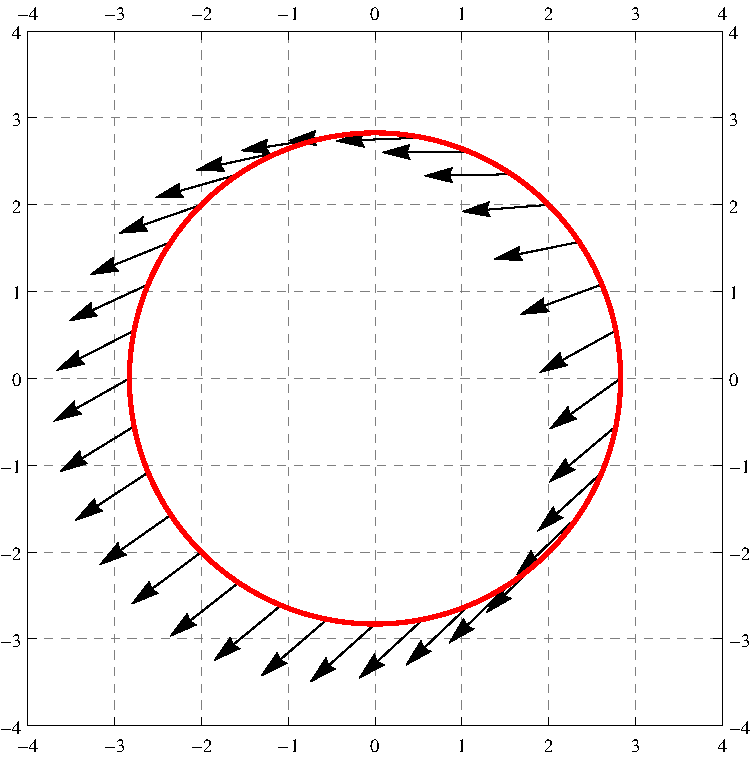
\includegraphics{curveVectors2.pdf}
  \end{image}
  Find the candidates for the maximum and minimum values for $F$ when
  restricted to $G(x,y) = c$.
  \begin{explanation}
    At the candidates for the extrema, we know that the gradient
    vector of $F$ must be
    \wordChoice{\choice{parallel}\choice[correct]{perpendicular}} to
    the curve $G(x,y) = c$. Hence we see that the points
    \[
    (x,y)\approx(\answer[given,tolerance=.5]{2.5},\answer[given,tolerance=.5]{.9})
    \]
    and
    \[
    (x,y)\approx (-2.3,\answer[given]{-1.7})
    \]
    are our candidates for extrema.
  \end{explanation}
\end{example}


\section{Working with algebra}

Let's work an example.

\begin{example}
  Let $F(x,y,z) = (1+x^2)(1+y^2)(1+z^2)$ and let $S$ the set:
  \[
  S = \{(x,y):x+y+z=1,\text{ where }x\ge 0, y\ge 0,z\ge 0\}
  \]
  Find the absolute maximum and minimum values of $F$ on $S$. This
  problem was a problem posed in the April $2004$ issue of \textit{Math
    Horizons}:
  \begin{explanation}
    We'll check the critical points of $F$. First compute $\grad F$:
    \[
    \grad F(x,y,z) = \vector{\answer[given]{2x(1+y^2)(1+z^2)},\answer[given]{2y(1+x^2)(1+z^2)},\answer[given]{2z(1+x^2)(1+y^2)}} 
    \]
    From this we see $\grad F = \vec{0}$ when
    \begin{align*}
      x &= \answer[given]{0}\\
      y &= \answer[given]{0}\\
      z &= \answer[given]{0}.
    \end{align*}
    Now we will set $G(x,y,z) = x+y+z$ and compute $\grad G$:
    \[
    \grad G(x,y,z) = \vector{\answer[given]{1},\answer[given]{1},\answer[given]{1}}
    \]
    We need to find points $(x,y,z)$ such that
    \[
    \grad F(x,y,z) = \lambda \cdot \grad G(x,y,z)
    \]
    for some number $\lambda$. Write with me
    \begin{align*}
      2x(1+y^2)(1+z^2) &=\lambda \cdot 1\\
      2y(1+x^2)(1+z^2) &=\lambda \cdot 1\\
      2z(1+x^2)(1+y^2) &=\lambda \cdot 1
    \end{align*}
    and
    \[
    x+y+z=1.
    \]
    Note the symmetry of the components of $\grad F$. From this we see that
    \[
    x = y = z.
    \]
    Hence
    \begin{align*}
    x+y+z&=1\\
    \answer[given]{3}x &= 1\\
    x &= \answer[given]{1/3}.
    \end{align*}
    Thus to find extrema for $F$ when restricted to $S$, we check the
    value of $F$ at the points:
    \[
    (0,0,0)\quad\text{and}\quad(1/3,1/3,1/3).
    \]
    Write with me
    \begin{align*}
      F(0,0,0) &= \answer[given]{1}\\
      F(1/3,1/3,1/3) &= \answer[given]{1000/729}
    \end{align*}
    We now see, via the Extreme Value Theorem, that the absolute
    maximum of $F$ when restricted to $S$ is given by
    \[
    (x,y,z) = (\answer[given]{1/3},\answer[given]{1/3},\answer[given]{1/3})
    \]
    and the absolute minimum is given by
    \[
    (x,y,z) = (\answer[given]{0},\answer[given]{0},\answer[given]{0}).
    \]
  \end{explanation}
\end{example}



\section{The Lagrangian}

Finally, we should point our that there are other ways to view
Lagrange multipliers.

\begin{definition}
  Given functions $F:\R^n\to\R$ and $G:\R^n\to\R$ the \dfn{Lagrangian} is the function
  \[
  \mathcal{L}(\vec{x},\lambda) = F(\vec{x}) - \lambda \cdot G(\vec{x}).
  \]
\end{definition}

Thus to check whether
\[
\grad F(\vec{x}) = \lambda \cdot \grad G(\vec{x})
\]
is equivalent to checking where
\[
\grad \mathcal{L}(\vec{x},\lambda) = \vec{0}
\]
or has undefined components. When working with constrained
optimization problems by hand, the Lagrangian doesn't help much, since
your next step is to look at 
\[
\grad \mathcal{L}(\vec{x},\lambda) = \vec{0}.
\]
However, there are certain advantages to working with the Lagrangian:
\begin{itemize}
\item If you are working with a computer, it might be better to work
  in terms of the Lagrangian, as there are efficient algorithms for
  checking when the gradient of the function is zero.
\item Working with the Lagrangian gives a method for changing
  ``constrained'' optimization to ``unconstrained'' optimization, as
  we are simply finding the critical points of
  $\mathcal{L}(\vec{x},\lambda)$.
\item The Lagrangian shows us a symmetry between $F$ and $G$.
\end{itemize}

For some interesting extra reading check out:
\begin{itemize}
\item \link[\textit{Lagrange Multipliers Can Fail to Determine
    Extrema}, J.\ Nunemacher, College Math Journal, January
  2003]{http://www.jstor.org/stable/3595848}.
\item \link[\textit{An ``Extremely'' Cautionary Tale}, M.\ Krusemeyer, College Math Journal, March 2000]{http://www.jstor.org/stable/2687586}.
\item \link[\textit{Unifying a Family of Extrema Problems},
  W.\ Barnier and D.\ Martin, College Math Journal, November
  1997]{http://www.jstor.org/stable/2687071}.
\end{itemize}







\end{document}





